

\tikzset{every picture/.style={line width=0.75pt}} %set default line width to 0.75pt        

\begin{tikzpicture}[x=0.75pt,y=0.75pt,yscale=-1,xscale=1]
%uncomment if require: \path (0,459); %set diagram left start at 0, and has height of 459

%Straight Lines [id:da3451988325670212] 
\draw [color={rgb, 255:red, 155; green, 155; blue, 155 }  ,draw opacity=1 ] [dash pattern={on 4.5pt off 4.5pt}]  (270,203) -- (270,358) ;
%Straight Lines [id:da1610923949227483] 
\draw [color={rgb, 255:red, 155; green, 155; blue, 155 }  ,draw opacity=1 ] [dash pattern={on 4.5pt off 4.5pt}]  (117,267) -- (270,267) ;
%Straight Lines [id:da4540475332681022] 
\draw [color={rgb, 255:red, 155; green, 155; blue, 155 }  ,draw opacity=1 ] [dash pattern={on 4.5pt off 4.5pt}]  (117,203) -- (270,203) ;
%Image [id:dp06244137649345305] 
\draw (321.5,278) node  {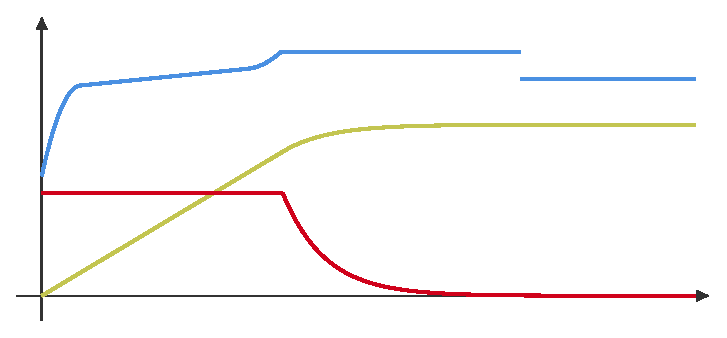
\includegraphics[width=332.25pt,height=145.5pt]{images/image_cccv}};
%Straight Lines [id:da8771255477316724] 
\draw [color={rgb, 255:red, 155; green, 155; blue, 155 }  ,draw opacity=1 ] [dash pattern={on 4.5pt off 4.5pt}]  (422,228.5) -- (422,360) ;
%Shape: Circle [id:dp0014709299474531257] 
\draw  [fill={rgb, 255:red, 255; green, 255; blue, 255 }  ,fill opacity=1 ] (268,203) .. controls (268,201.9) and (268.9,201) .. (270,201) .. controls (271.1,201) and (272,201.9) .. (272,203) .. controls (272,204.1) and (271.1,205) .. (270,205) .. controls (268.9,205) and (268,204.1) .. (268,203) -- cycle ;
%Shape: Circle [id:dp8257690320080588] 
\draw  [fill={rgb, 255:red, 255; green, 255; blue, 255 }  ,fill opacity=1 ] (268,267) .. controls (268,265.9) and (268.9,265) .. (270,265) .. controls (271.1,265) and (272,265.9) .. (272,267) .. controls (272,268.1) and (271.1,269) .. (270,269) .. controls (268.9,269) and (268,268.1) .. (268,267) -- cycle ;
%Straight Lines [id:da48605435215358694] 
\draw [color={rgb, 255:red, 74; green, 144; blue, 226 }  ,draw opacity=1 ][line width=1.5]  [dash pattern={on 1.69pt off 2.76pt}]  (422,207.7) -- (422,217.2) ;
%Straight Lines [id:da6398477641060736] 
\draw    (272,399) -- (420,399) ;
\draw [shift={(422,399)}, rotate = 180] [color={rgb, 255:red, 0; green, 0; blue, 0 }  ][line width=0.75]    (10.93,-3.29) .. controls (6.95,-1.4) and (3.31,-0.3) .. (0,0) .. controls (3.31,0.3) and (6.95,1.4) .. (10.93,3.29)   ;
\draw [shift={(270,399)}, rotate = 0] [color={rgb, 255:red, 0; green, 0; blue, 0 }  ][line width=0.75]    (10.93,-3.29) .. controls (6.95,-1.4) and (3.31,-0.3) .. (0,0) .. controls (3.31,0.3) and (6.95,1.4) .. (10.93,3.29)   ;
%Straight Lines [id:da7717485329022031] 
\draw    (118.5,399) -- (268,399) ;
\draw [shift={(270,399)}, rotate = 180] [color={rgb, 255:red, 0; green, 0; blue, 0 }  ][line width=0.75]    (10.93,-3.29) .. controls (6.95,-1.4) and (3.31,-0.3) .. (0,0) .. controls (3.31,0.3) and (6.95,1.4) .. (10.93,3.29)   ;
\draw [shift={(116.5,399)}, rotate = 0] [color={rgb, 255:red, 0; green, 0; blue, 0 }  ][line width=0.75]    (10.93,-3.29) .. controls (6.95,-1.4) and (3.31,-0.3) .. (0,0) .. controls (3.31,0.3) and (6.95,1.4) .. (10.93,3.29)   ;
%Straight Lines [id:da8998950689600032] 
\draw    (116,394) -- (116,404) ;
%Straight Lines [id:da17048346486898192] 
\draw    (270,394) -- (270,404) ;
%Straight Lines [id:da8039553388960854] 
\draw    (422,394) -- (422,404) ;
%Straight Lines [id:da2911914982770165] 
\draw [color={rgb, 255:red, 74; green, 144; blue, 226 }  ,draw opacity=1 ]   (78,124) -- (103,124) ;
%Straight Lines [id:da500593174587459] 
\draw [color={rgb, 255:red, 208; green, 2; blue, 27 }  ,draw opacity=1 ]   (78,144) -- (103,144) ;
%Straight Lines [id:da47080918502581004] 
\draw [color={rgb, 255:red, 195; green, 197; blue, 81 }  ,draw opacity=1 ]   (78,164) -- (103,164) ;

%Straight Lines [id:da7924785218065409] 
\draw [color={rgb, 255:red, 155; green, 155; blue, 155 }  ,draw opacity=1 ] [dash pattern={on 4.5pt off 4.5pt}]  (117,249) -- (533,249) ;

% Text Node
\draw (106,117.4) node [anchor=north west][inner sep=0.75pt]  [font=\footnotesize]  {$U_{\mathrm{B}}( t)$};
% Text Node
\draw (106,137.4) node [anchor=north west][inner sep=0.75pt]  [font=\footnotesize]  {$I_{\mathrm{B}}( t)$};
% Text Node
\draw (106,157.4) node [anchor=north west][inner sep=0.75pt]  [font=\footnotesize]  {$Q_{\mathrm{B}}( t)$};
% Text Node
\draw (547,352.4) node [anchor=north west][inner sep=0.75pt]  [font=\footnotesize]  {$t$};
% Text Node
\draw (142,382) node [anchor=north west][inner sep=0.75pt]  [font=\footnotesize] [align=left] {Constant current};
% Text Node
\draw (294,382) node [anchor=north west][inner sep=0.75pt]  [font=\footnotesize] [align=left] {Constant voltage};
% Text Node
\draw (102,363.4) node [anchor=north west][inner sep=0.75pt]  [font=\footnotesize]  {$0$};
% Text Node
\draw (84.5,242.4) node [anchor=north west][inner sep=0.75pt]  [font=\footnotesize]  {$Q_{\mathrm{tot}}$};
% Text Node
\draw (87,198.4) node [anchor=north west][inner sep=0.75pt]  [font=\scriptsize]  {$U_{\mathrm{full}}$};
% Text Node
\draw (97.2,287.4) node [anchor=north west][inner sep=0.75pt]  [font=\scriptsize]  {$I_{\mathrm{C}}$};
% Text Node
\draw (263,362.4) node [anchor=north west][inner sep=0.75pt]  [font=\footnotesize]  {$t_{\mathrm{C}}$};
% Text Node
\draw (400,362.4) node [anchor=north west][inner sep=0.75pt]  [font=\footnotesize]  {$t_{\mathrm{C}} +t_{\mathrm{V}}$};
% Text Node
\draw (60.5,259.4) node [anchor=north west][inner sep=0.75pt]  [font=\footnotesize]  {$Q_{\mathrm{B}}( t_{\mathrm{CC}})$};


\end{tikzpicture}





